\chapter{Software}\label{kap6}
Dieses Kapitel behandelt das zum Einsatz kommende Softwaresystem in Hinblick auf die verwendete Toolchain, die Programmstruktur als solche und Optimierungspotentiale. Dadurch soll dem Leser ein Überblick gegeben werden, sodass dieser den Programmablauf nachvollziehen kann und selbstständig Weiterentwicklungen durchführen kann.

\section{Toolchain}
Unter Toolchain werden die Werkzeuge bzw. Programme und ihr Zusammenwirken bezeichnet, die zur Programmentwicklung verwendet werden.\\ Für die vorliegende Aufgabenstellung ist ein Programm notwendig, das auf einem Mikrocontroller des Typs STM32F4 lauffähig ist. Zur Entwicklung des Programms kommt ein innovativer Ansatz zum Einsatz, der einfach verständlich und schnell erlernbar ist. Er basiert auf \textit{Matlab Simulink} und ermöglicht die Programmierung des Mikrocontrollers auf intuitive Weise. Um hardwarespezifische Blöcke bspw. zum Auslesen der ADCs benutzen zu können, wird ein Simulink Blockset namens \textit{Waijung} eingesetzt \autoref{waijung}. Um das Blockschaltbild für den STM32 ausführbar zu machen, wird neben Simulink selbst auch der \textit{Simulink Coder} und der \textit{Embedded Coder} für Matlab benötigt. Durch diese Toolboxes ist es möglich aus einem Simulink Modell  C-Code zu generieren\autoref{simulinkCoder}. Der \textit{Embedded Coder} führt dabei zusätzlich Optimierungen durch, die eine effiziente Ausführung auf einem eingebettetem System ermöglichen \autoref{embeddedCoder}. 
Auch dieser C-Code ist nicht direkt ausführbar auf einem ARM-basierten Prozessor, wie es der STM32F4 ist. Es existieren jedoch geeignete Übersetzungstools (Compiler), die den C-Code in ARM-Assembler übersetzen und direkt lauffähig machen können. Im \textit{Waijung Blockset} werden dafür die \textit{GNU Tools for ARM embedded processors} mitgeliefert. Der kompilierte Code muss im letzten Schritt auf den Mikrocontroller übertragen werden, auch \textit{flashen} oder \textit{programmieren} genannt. Die Firma ST liefert dafür ein Programm namens \textit{STLink Utility}, welches neben des Programmiervorgangs über die definierte Programmierschnittstelle SWD auch Debugging-Fähigkeiten liefert, womit Fehlerzustände lokalisiert und beseitigt werden können. Einen groben Überblick über den Prozess vom Simulink  Modell bis zur Ausführung auf der Zielhardware wird in \autoref{fig_toolchain} gegeben.

\begin{figure}[H]%
\centering
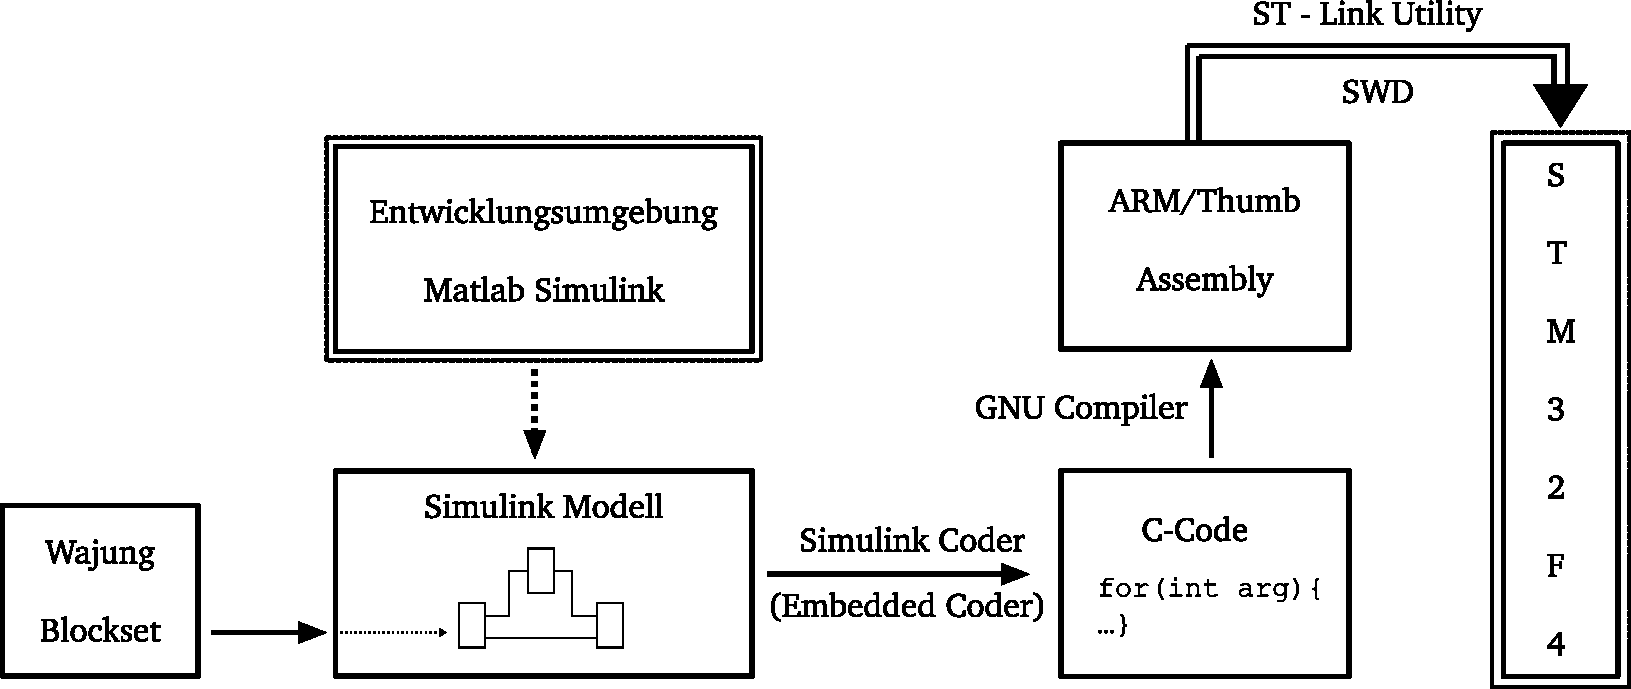
\includegraphics[width=0.8\columnwidth]{./Bilder/fig_toolchain}%
\caption{Vereinfachte Darstellung der eingesetzten Toolchain}%
\label{fig_toolchain}%
\end{figure}

\section{Vorstellung des Hauptprogramms}
Um einen Einblick in das Hauptprogramm zu bieten, das auf dem finalen \textit{smart-actuator} zum Einsatz kommt, wird zunächst geklärt welche Systemarchitektur zum Einsatz kommt.
Insbesondere im Gebiet des \textit{automated driving} sind viele Architekturansätze bekannt, durch welche komplexe Software strukturierter, robuster und zuverlässiger werden soll \cite{automated}. Weit verbreitet ist die 1983 entwickelte Architektur von Rasmussen, die zwischen wissensbasiertem, regelbasiertem und reflexbasiertem Verhalten unterscheidet. Unter reflexbasiertem Verhalten werden Aktionen verstanden, die rein reaktiv Sensordaten in Aktor-Aktivitäten umsetzen, ohne dabei komplexen Regeln zu folgen. Regelbasiertes Verhalten auf der anderen Seite ist bestimmt durch feste vordefinierte Regeln, die auf bestimmte Situationen angewendet werden. Falls eine Situation jedoch nicht vorhersehbar ist bzw. keine Regeln dafür hinterlegt sind, muss durch wissensbasiertes Verhalten gehandelt werden \cite{automated}. Dieses Verhalten kann beispielsweise durch neuronale Netze erreicht werden, die jedoch in dieser Arbeit keine Anwendung finden. \autoref{Rasmussen 83}\\
Wichtig sind daher die unteren beiden Ebenen, wobei nur die reflexbasierte Ebene Zugriff auf Sensorik und Aktorik hat. Auf übergeordneter regelbasierter Ebene werden dann vorverarbeitete Werte ausgewertet und anhand fester Regeln Handlungsanweisungen an die untere Ebene erzeugt. In \autoref{fig_arch} ist die Architektur nochmal vereinfacht dargestellt.
\begin{figure}%
\centering
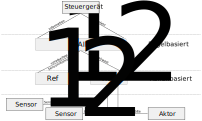
\includegraphics[width=0.8\columnwidth]{./Bilder/fig_arch}%
\caption{Drei-Ebenenarchitektur nach Rasmussen (vereinfacht)}%
\label{fig_arch}%
\end{figure}
Eine regelbasierte Hauptkomponente (MAIN) entscheidet je nach anliegenden vorverarbeiteten Sensorinformationen und Steuerbefehlen des übergeordneten Steuergeräts, welches Verhalten auf Reflexebene erwünscht ist. Es wird beispielsweise eine Sollgröße für einen Regler ($Ref_{2}$) vorgegeben, die schnellstmöglich ausgeregelt wird. \\
Konkret wird die Hauptkomponente durch einen Zustandsautomaten realisiert, der mehrere Ein- und Ausgänge zu anderen Komponenten bietet. Die Außendarstellung ist in \autoref{fig_main} dargestellt. Dabei sind links Eingänge von Sensorik- und CAN-Komponenten angeordnet und rechts Ausgänge. Die erste Buchstabenfolge beschreibt dabei jeweils von welchem Block das Signal ursprünglich generiert wird. Die Abkürzungen sind in \autoref{tab_kurz} erläutert. \\
Ein Vorteil dieser Architektur ist zunächst die Übersichtlichkeit und Nachvollziehbarkeit, da der gesamte Programmablauf in der Hauptkomponente nachvollzogen werden kann. Wie genau nämlich die Anweisungen dieser Hauptkomponente umgesetzt werden, ist für das Verständnis irrelevant. Darüber hinaus ist der wichtigste Vorteil, dass durch die strikte Trennung zwischen regelbasierter und reflexbasierter Ebene unterschiedliche Arbeitsfrequenzen realisiert werden können. Die aufwändige regelbasierte Ebene arbeitet dabei in der Regel langsamer. Weiterhin gelten die allgemeinen Vorteile beim Einsatz einer definierten Architektur wie Robustheit, Zuverlässigkeit, Wartbarkeit. Als Nachteilig ist anzusehen, dass sich der Entwickler durch die Anwendung dieser Architektur einschränkt und daher ggf. nicht zum idealen Ergebnis kommt. \autoref{} \\
Eine klassische alternative Struktur stellt die \textit{Real-Time Control System Architecture} nach \autoref{albus} dar. Diese besitzt ein breites Anwendungsspektrum, ist jedoch durch eine größere Anzahl an Ebenen komplexer und wird vornehmlich für intelligente Regelungen in unbekanntem Umfeld eingesetzt. \autoref{ James S. Albus (1992). A Reference Model Architecture for Intelligent Systems Design 2008-09-16 at the Wayback Machine Intelligent Systems Division, Manufacturing Engineering Laboratory, National Institute of Standards and Technology.}
\begin{table}%
\centering
\begin{tabular}{c c}
\hline
Abkürzung & Erläuterung \\
\hline
POS & Schaltgabelpositionsermittlung\\
CAN & CAN - Schnittstelle\\
CAL & Kalibrierung des Lagesensors\\
ERR & Fehlererkennung\\
MAIN & Hauptzustandsautomat\\
SEN & Sensorik\\
CONS & Regler zum Schalten\\
CONH & Regler zum Positionshalten\\
PWM & Auswahlglied für PWM-Signal\\
MOT & Motortreiber \\

\end{tabular}
\caption{Erläuterung der Abkürzungen im Softwaresystem}
\label{tab_kurz}
\end{table} 

\subsection{Gesamtsystem}
In \autoref{fig_gesamtsystem} ist das gesamte Softwaresystem dargestellt. Hierbei ist die Sensorik hellblau, die Regelung hellgrün, die Aktorik dunkelgrün, die CAN-Kommunikation gelb und die Fehlererkennung orange dargestellt. Alle Komponenten agieren reflexbasiert direkt auf die Steuerungssignale des mittig angeordneten Hauptzustandsautomaten. Eine Ausnahme bildet die Kalibrierung, die ihrerseits durch einen Zustandsautomaten realisiert ist, wobei dieser durch den Hauptzustandsautomaten aktiviert und gestoppt wird. 
\begin{figure}[H]%
\centering
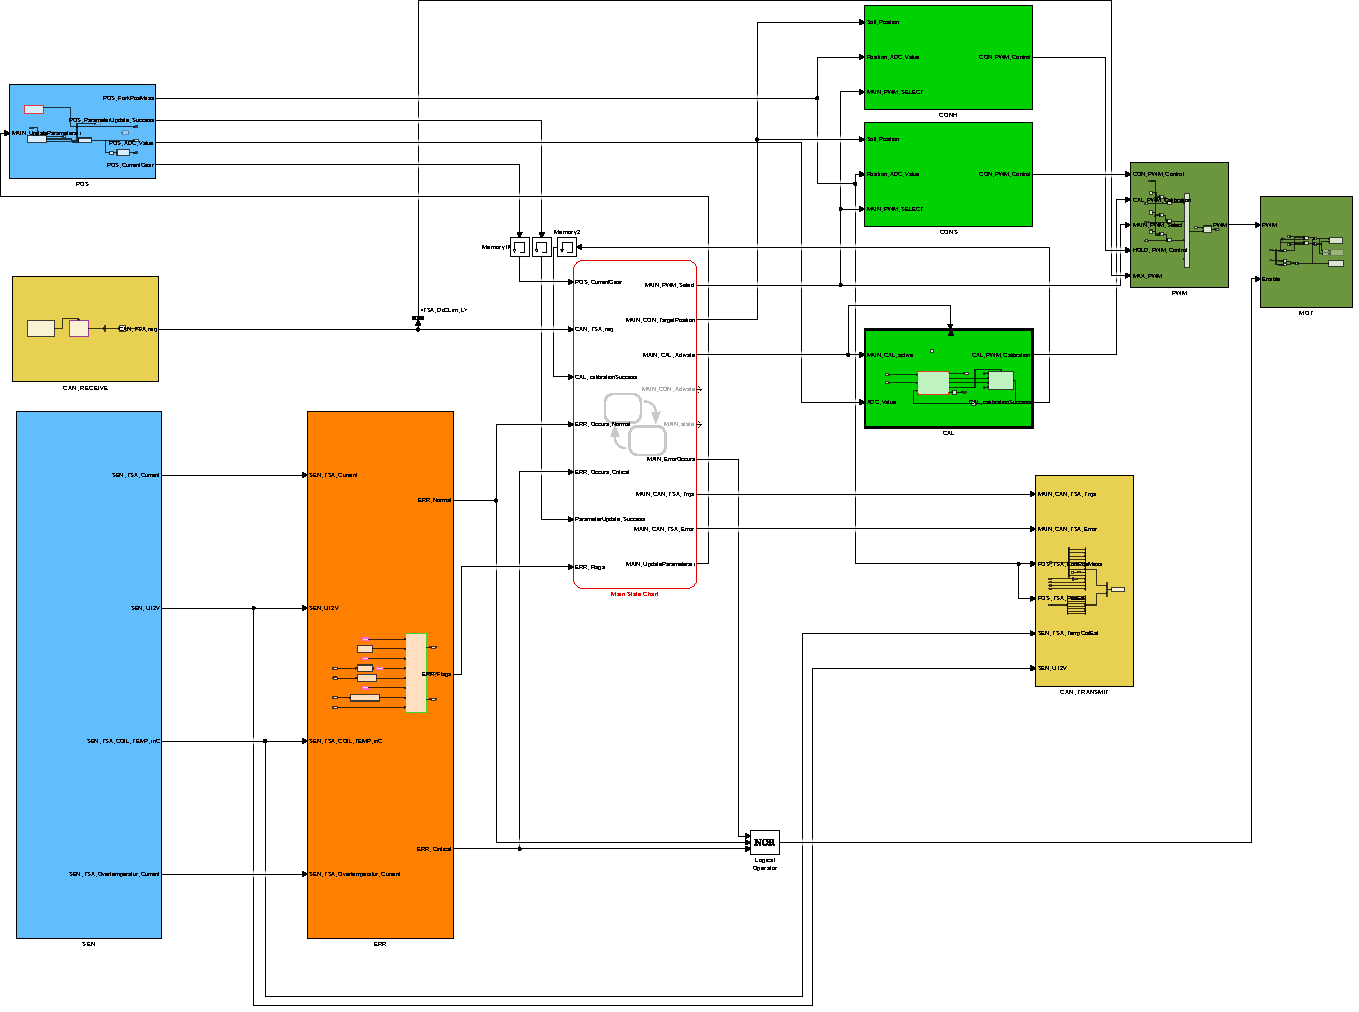
\includegraphics[width=0.9\columnwidth]{./Bilder/fig_gesamtsystem}%
\caption{Darstellung des Gesamtsystems}%
\label{fig_gesamtsystem}%
\end{figure}
Im Folgenden wird der Hauptzustandsautomat und die reflexbasierten Komponenten einzeln erläutert.

\subsection{Hauptzustandsautomat (MAIN)}

\begin{figure}[H]%
\centering
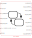
\includegraphics[width=0.4\columnwidth]{./Bilder/fig_main}%
\caption{Hauptzustandsautomat (MAIN), Außenansicht}%
\label{fig_main}%
\end{figure}

Der Hauptzustandsautomat ist die Kernkomponente der Software und beeinflusst jede Komponente des Systems. Als Eingangssignal wird dem Hauptzustandsautomaten
\begin{itemize}
	\item der aktuell eingelegte Gang (\textit{POS\_CurrentGear}),
	\item die letzte empfangene CAN-Nachricht (\textit{CAN\_TSA\_req}),
	\item das Statussignal einer laufenden/abgeschlossenen Kalibrierung (\textit{CAL\_calibrationSuccess}),
	\item das Fehlersignal bei \textit{normalen Fehlern} (\textit{ERR\_Occurs\_Normal}),
	\item das Fehlersignal bei \textit{kritischen Fehlern} (\textit{ERR\_Occurs\_Ciritcal}),
	\item das Statussignal beim Laden der Kalibrierparameter (\textit{ParameterUpdate\_Success}) und
	\item eine Liste an Fehler Bits (\textit{ERR\_Flags})
\end{itemize}
zugeführt. Als Ausgangssignal gibt der Hauptzustandsautomat
\begin{itemize}
	\item die aktuelle Quelle für PWM Generierung (\textit{MAIN\_PWM\_Select}),
	\item den Wunschgang,
	\item das Aktivierungssignal der Kalibrierung,
	\item den aktuellen Zustand des Automaten,
	\item ein Fehlersignal bei internem Fehler im Automaten,
	\item die \textit{Trqs}-CAN-Nachricht (siehe \autoref{CAN_Nachrichten}),
	\item die \textit{Error}-CAN-Nachricht (siehe \autoref{CAN_Nachrichten}) und
	\item den Auslöser zum Auslesen der Kalibrierparameter
\end{itemize}
aus. Über \textit{MAIN\_PWM\_Select} wird nicht nur die Quelle ausgewählt, die den Motortreiber ansteuert, sondern ebenfalls welche Teilsysteme aktiv sind. Somit wird sichergestellt, dass zu jedem Zeitpunkt ausschließlich ein einziger Regelalgorithmus oder Kalibrieralgorithmus ausgeführt wird (siehe dazu auch \autoref{performanceopt}).\\
Intern agiert der Zustandsautomat in vier streng separierten Betriebsmodi. Nach jedem Reset (bspw. nach dem Anlegen der Versorgungsspannung) befindet sich der Automat zunächst im Initialisierungsschritt. Hier werden zunächst für die Ausführung relevante Variablen initialisiert. Daran anschließend werden die Kalibrierparameter aus dem nichtflüchtigen Speicher geladen. Das Auslesen und Zwischenspeichern der Werte findet dabei im Block zur Schaltgabelpositionsermittlung (POS) statt und wird durch das Setzen eines entsprechenden Triggersignals angestoßen. Durch die Kalibrierwerte ist es nun möglich die aktuelle Schaltgabelposition zu bestimmen, wobei zunächst im Betriebsmodus \textbf{Inaktiv} verblieben wird. Durch einen entsprechenden CAN-Befehl kann der Übergang in den Betriebsmodus \textbf{Regulär} erfolgen. Hierin ist es möglich Schaltbefehle auszuführen. Es wird unterschieden zwischen \textit{Schalte in Gang X} und \textit{Bleibe in Gang X}, wobei jeweils entweder der Regler zum Schalten oder der Regler zum Halten der Position aktiv ist. Für Letzteren existiert noch keine zufriedenstellende Realisierung. Falls eine Kalibrierung durchgeführt werden soll, kann aus diesem Betriebsmodus in den Betriebsmodus \textbf{Kalibrierung} gewechselt werden. Aus allen Betriebsmodi wird durch das Auftreten eines Fehlers (angezeigt durch die entsprechenden Eingangssignale am Automaten) direkt in den Betriebsmodus \textbf{Fehler} übergegangen. In diesem Betriebsmodus werden keine Stellgrößen am Motortreiber zugelassen und alle Regler sind deaktiviert. Erst durch das Senden des entsprechenden Freigabe-Befehls wird wieder in den Betriebsmodus \textbf{Inaktiv} geschaltet.
 
\begin{figure}[H]%
\centering
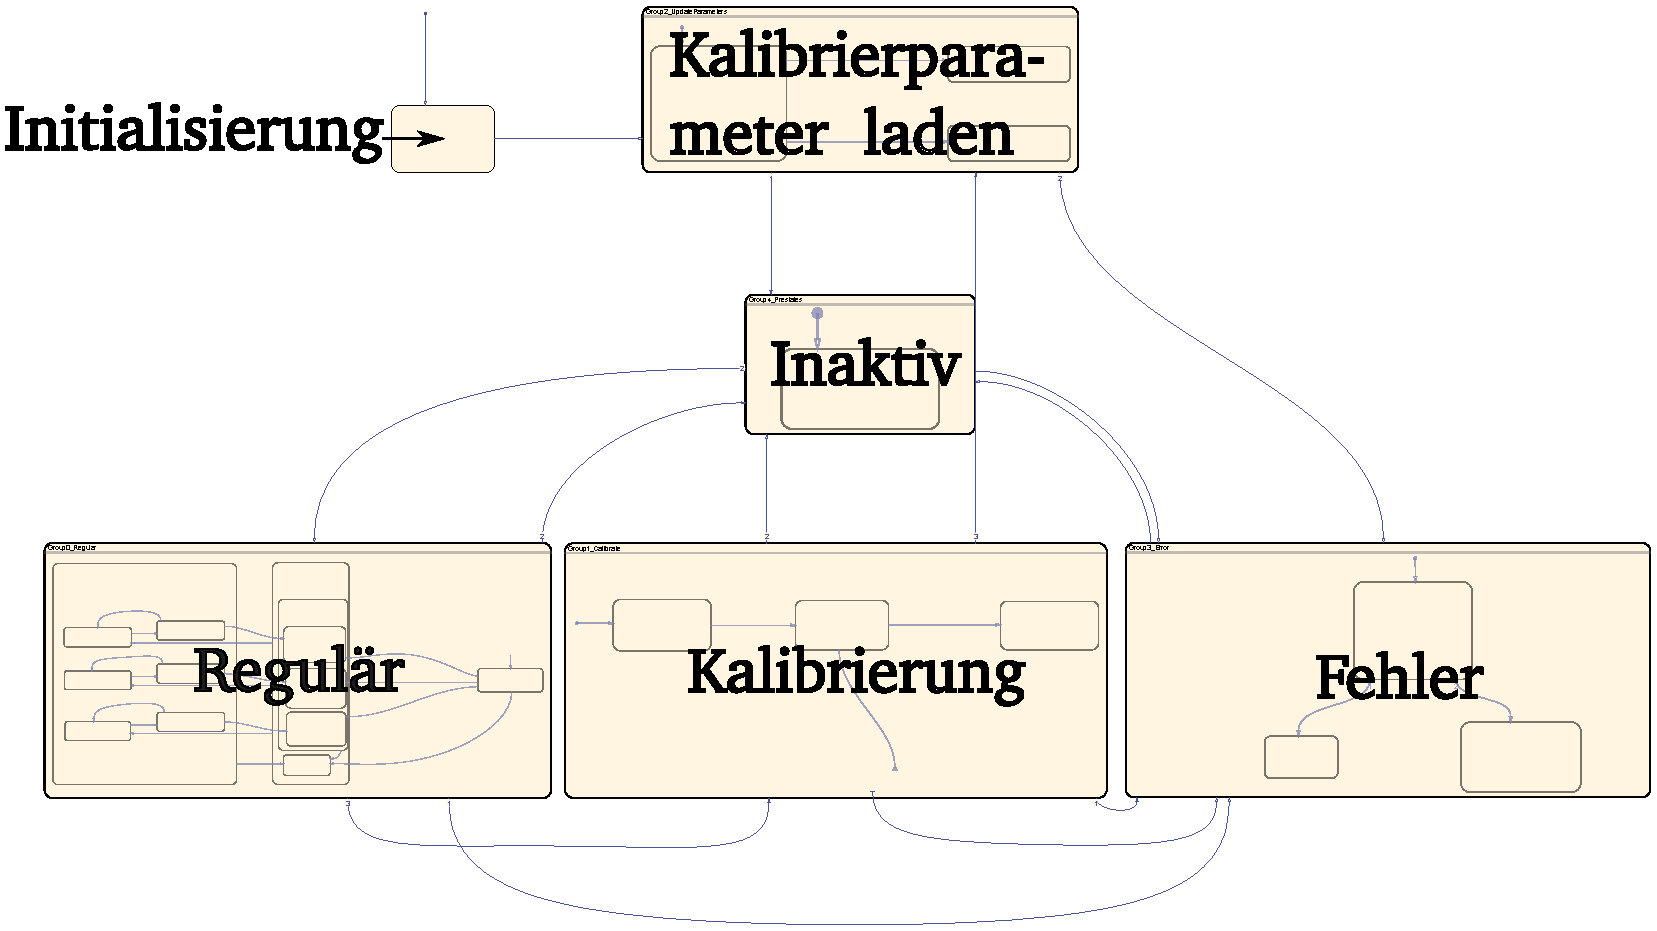
\includegraphics[width=0.6\columnwidth]{./Bilder/fig_main_detail}%
\caption{Hauptzustandsautomat (MAIN), vereinfachter Aufbau}%
\label{fig_main_detail}%
\end{figure}

\subsection{Positionsermittlung (POS)}\label{lagesens}
\begin{figure}[H]%
\centering
\includegraphics[width=0.3\columnwidth]{./Bilder/fig_POS}%
\caption{Schaltgabelpositionsermittlung}%
\label{fig_POS}%
\end{figure}

Die Positionsermittlung der Schaltgabel genießt eine Sonderstellung unter der Sensorik. Sie stellt die Regelgröße dar und ist daher von essentieller Bedeutung für die Regelung.  Dementsprechend wird die Positionsregelung getrennt von der restlichen Sensorik behandelt. Die Sensorik ist im \textit{SEN}-Subsystem anzutreffen (siehe \autoref{SEN}). Eingangsseitig kann durch den Hauptzustandsautomaten angestoßen werden, dass die Kalibrierdaten für die Lagesensorik aus dem nichtflüchtigen Speicher gelesen werden. Ausgangsseitig wird 
\begin{itemize}
	\item die momentane Gabelposition in Millimetern,
	\item der Zustand des Lesezugriffs auf die Kalibrierdaten,
	\item die Sensor Rohdaten und 
	\item der aktuell eingelegte Gang
\end{itemize}
bereit gestellt. 
Die Positionsmessung wird intern über einen ADC realisiert, durch den die Ausgangsspannung des Hall-Sensors (vlg. \autoref{regler}) in die Schaltgabelposition übersetzt wird. Um die Genauigkeit zu erhöhen wird sowohl der direkte als auch der komplementäre Sensorausgang erfasst. Somit wird eine Genauigkeit von \SI{0,1}{mm} erzielt. Durch eine \textit{Burst}-Messung kann die Genauigkeit noch weiter erhöht werden. Hierbei werden mehrere Messungen durchgeführt und in einen Puffer zwischengespeichert ohne den Programmablauf zu unterbrechen. In regelmäßiger Auslesefrequenz wird die gepufferte Menge an Sensordaten durch das Programm ausgelesen und verarbeitet. Im STM32 wird diese Funktion über \textit{Direct Memory Access} realisiert, wodurch die ADC-Peripherie Messwerte direkt in den Speicher schreibt, den der Prozessor in regelmäßigen Abständen ausließt \autoref{stm32}. Diese Funktion wird in \autoref{perfVergl} wieder aufgegriffen.

\subsection{CAN-Kommunikation (CAN)}

\begin{figure}[H]%
\centering
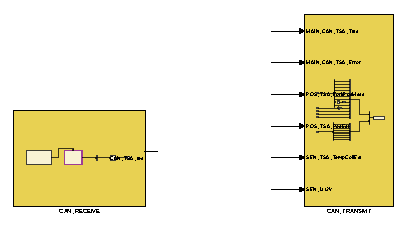
\includegraphics[width=0.6\columnwidth]{./Bilder/fig_can}%
\caption{CAN-Kommunikation}%
\label{fig_can}%
\end{figure}

Die CAN-Kommunikation wird durch eine Empfangskomponente (\textit{receive}) und eine Sendekomponente (\textit{transmit}) realisiert. Die Empfangskomponente funktioniert Interrupt-basiert und wird somit immer aktiv, wenn eine neue Nachricht empfangen wird. Über einen Rate-Transmission-Block wird diese Empfangsfrequenz an die Arbeitsfrequenz des Hauptzustandsautomaten angepasst. Als Ausgang steht dem Automaten ein Bus-Vektor mit dem Nachrichteninhalt zur Verfügung. 
Die Sendekomponente basiert auf \textit{Non-Blocking}-Basis. Dadurch können während des Sendevorgangs nebenläufig auch noch andere Aufgaben abgearbeitet werden. Die einzelnen Eingangswerte werden vor dem Senden zu größeren Nachrichten zusammengefügt.

\subsection{Sensorik (SEN)}\label{SEN}
\begin{figure}[H]%
\centering
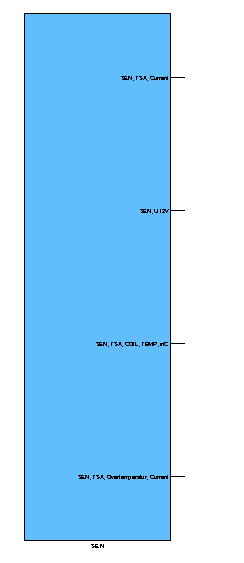
\includegraphics[width=0.2\columnwidth]{./Bilder/fig_sen}%
\caption{Sensorik}%
\label{fig_sen}%
\end{figure}
Die Sensorik umfasst eine Strommessung durch den Aktor, eine Spannungsmessung am Eingang, eine Spulentemperaturmessung und eine Detektion gegen Übertemperatur/Überstrom an den Halbbrücken. Die Sensorwerte stehen zunächst als ADC-Rohwerte für die weitere Verarbeitung bereit. Diese werden je nach Sensortyp skaliert oder wie im Falle des externen Thermistors durch komplexe Formeln in den realen Messwert konvertiert (vgl. \autoref{ch:komp}). An den Ausgängen stehen anschließend die Messgrößen in gewünschter Einheit bereit. Der Lagesensor wird nach \autoref{lagesens} implementiert.

\subsection{Fehlererkennung (ERR)}
\begin{figure}[H]%
\centering
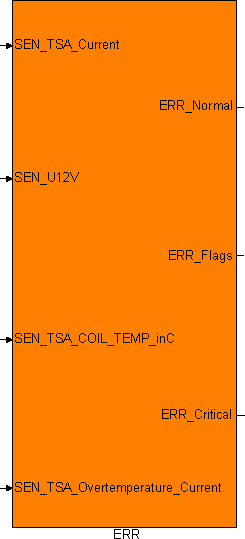
\includegraphics[width=0.2\columnwidth]{./Bilder/fig_err}%
\caption{Fehlererkennung}%
\label{fig_err}%
\end{figure}
Durch die Fehlererkennung werden die gemessenen Überwachungsgrößen mit Schwellwerten verglichen und ggf. ein Fehlersignal zum Hauptzustandsautomaten weitergeleitet. Dabei muss berücksichtigt werden, dass Messfehler erkannt und ggf. gefiltert werden und nicht zu falsch positiv Ergebnissen führen. Auf der anderen Seite sollten Fehler schnellstmöglich erkannt werden und die falsch negativ - Rate minimal sein. Neben dem Hauptzustandsautomaten besitzt die Komponente auch noch eine Schnittstelle zum Motortreiber, um den Stromfluss im Aktor schnellstmöglich zu unterbinden. Hierfür wird das in \autoref{subsec:MOT} genauer erklärte \textit{enable}-Signale genutzt.

\subsection{Kalibrierung (CAL)}

\begin{figure}[H]%
\centering
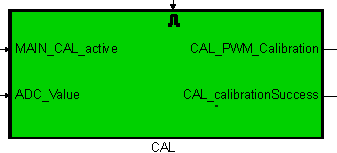
\includegraphics[width=0.3\columnwidth]{./Bilder/fig_cal}%
\caption{Kalibrierung (Lagesensor)}%
\label{fig_cal}%
\end{figure}

Die Kalibrierung dient dazu, den Spannungswerten des Lagesensors konkrete Positionen der Schaltgabel zuordnen zu können. Das Kalibrierungsverfahren basiert auf dem Ansatz von \cite{VorgaengerADP}. Es werden dabei die Anschlagspositionen durch große Stellgrößen angefahren und der Sensor an diesen Werten ausgelesen. Nach mehrmaliger Ausführung und anschließender Mittlung werden die Kalibrierungswerte nichtflüchtig abgespeichert. Im Falle eines Spannungsverlustes stehen die Kalibrierungsdaten nach wie vor bereit. Die Komponente besitzt Schnittstellen zur Lagesensorik sowie zum Hauptzustandsautomaten, von welchem aus die Kalibrierung eingeleitet wird.

\subsection{Halteregler (CONH) und Schaltregler (CONS)}

\begin{figure}[H]%
\centering
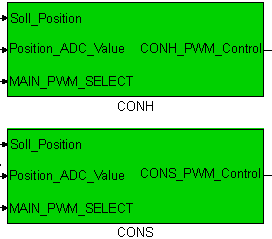
\includegraphics[width=0.2\columnwidth]{./Bilder/fig_conh_cons}%
\caption{Regelung}%
\label{fig_conh_cons}%
\end{figure}

Für die Regelung der Schaltgabelposition nach \autoref{regler} werden den Reglern die momentane Gabelpositon zugeführt. Darüber hinaus wird über den Hauptzustandsautomaten die Sollposition vorgegeben. Über den Soll-Ist-Vergleich und die Anwendung eines Regelgesetzes wird schließlich eine PWM als Stellgröße ermittelt. Eine Regelfrequenz von \SI{10}{kHz} hat sich als ausreichend schnell herausgestellt und kann durch den Mikrocontroller geleistet werden. Beim \textit{Schaltregler} kommt ein PID-Regler mit Störgrößenkompensation zum Einsatz, der in \cite{VorgaengerADP} erarbeitet wurde. Eine praktikable Lösung für einen \textit{Halteregler} konnte nicht ermittelt werden. Der jeweilige Regler ist nur aktiv, falls er durch den \textit{MAIN\_PWM\_SELECT} des Hauptzustandsautomaten auch explizit angefragt ist.
 
\subsection{Auswahlglied für PWM-Signal (PWM)}

\begin{figure}[H]%
\centering
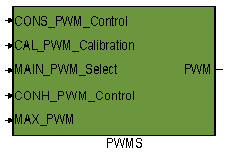
\includegraphics[width=0.2\columnwidth]{./Bilder/fig_pwm}%
\caption{Auswahlglied für PWM-Signal}%
\label{fig_pwm}%
\end{figure}

Über das Auswahlglied für das PWM-Signal wird selektiert, welche der möglichen PWM-Signale zum Motortreiber durchgeschaltet wird. Die Auswahl wird aufgrund des \textit{MAIN\_PWM\_SELECT}-Eingangs getroffen. Darüber hinaus kann die maximale PWM durch entsprechende CAN-Signale begrenzt werden. 

\subsection{Motortreiber (MOT)} \label{subsec:MOT}

\begin{figure}[H]%
\centering
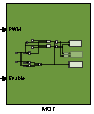
\includegraphics[width=0.2\columnwidth]{./Bilder/fig_mot}%
\caption{Motortreiber}%
\label{fig_mot}%
\end{figure}

Der Motortreiber erwartet ein vorgegebenes PWM-Signal, bzw. dessen Tastgrad \textit{p} (vgl. \autoref{sec:PWM_kap2}). Über das Vorzeichen wird bestimmt, welche der beiden H-Brücken gepulst angesteuert wird und welche konstant auf Erdpotential gesetzt wird. Über ein explizites \textit{nable}-Signal kann der Motortreiber bspw. im Falle einer Notausschaltung deaktiviert werden. Hierfür wird der Motortreiber über einen separaten Pin in einen \textit{sleep-mode} gesetzt (vgl. \autoref{sec:hbridge}). Zwei Vorgabewerte werden demnach in Signale umgewandelt, die zur H-Brücke weitergeführt werden.


\section{Codegenerierung und Performanceoptimierung} \label{performanceopt}
Der generierte und kompilierte Code wird auf dem Mikroprozessor Cortex M4 ausgeführt, der auf dem STM32F4 eingesetzt wird. Dieser Mikroprozessor zeichnet sich durch eine vergleichsweise hohe Rechenleistung aus und verfügt darüber hinaus über eine \textit{Floating Point Unit} (FPU). Somit ist er in der Lage Gleitkommazahlen zu verrechnen. Bei maximaler Taktfrequenz ist die Rechenleistung begrenzt auf \SI{225}{DMIPS}. In DMIPS wird dabei die Leistungsfähigkeit, gemessen an einem repräsentativen Testprogramm namens \textit{Dhrystone}, angegeben \cite{https://www.itwissen.info/DMIPS-Dhrystone-MIPS.html}. Der Prozessor kann daher nicht beliebig viele Aufgaben in beliebiger Arbeitsfrequenz abarbeiten. Für weiterführende Informationen sei auf das Datenblatt \cite{stm32} verwiesen.\\
Um zu verstehen, wie die begrenzten Rechenressourcen optimal ausgelastet werden können, ist es von Vorteil den Codegenerierungsprozess zu kennen. Über Waijung und die Simulink Toolboxes wird Code nach dem sogenannten \textit{Multirate Single Tasking}- Prinzip generiert. Somit ist es möglich, mehrere Aufgaben mit unterschiedlichen Arbeitsfrequenzen abzuarbeiten. Über den sogenannten \textit{SysTick Timer} wird in der Frequenz der höchstfrequenten Aufgabe ein Interrupt ausgelöst. Ein Interrupt bezeichnet eine Unterbrechung des regulären Programmablaufs, wobei nach der Abarbeitung der sogenannten Interrupt Service Routine wieder der reguläre Programmablauf an der letzten Stelle fortgeführt wird. 
Innerhalb des \textit{SysTick Timer}-Interrupts wird angestoßen, dass diejenigen Aufgaben ausgeführt werden, die zum entsprechenden Zeitpunkt ausgeführt werden sollen. Beispielsweise wird eine Aufgabe, die mit \SI{100}{Hz} ausgeführt werden soll, durch jeden zehnten \textit{SysTick Timer}-Interrupt mit \SI{1}{kHz} angestoßen. Eine Besonderheit fallen Aufgaben zu, die als laufzeitkritisch eingestuft werden, denn diese Aufgaben werden direkt innerhalb der Interrupt Service Routine abgearbeitet und haben somit Priorität vor den übrigen Aufgaben. Ein Beispiel einer solchen Aufgabe ist der geschlossene Regelkreis zur Reglung der Gabelposition. Um den Ablauf des Programms nicht zu gefährden, muss darauf geachtet werden, dass diese Aufgaben nicht länger dauern als bis zum Auslösen des nächsten \textit{SysTick Timer}-Interrupts. Zusätzlich muss noch genügend Zeit bleiben, um die übrigen Aufgaben auszuführen.\cite{waijung}\\
Um dies zu ermöglichen wird eine Reihe von Maßnahmen ergriffen, die im Folgenden kurz vorgestellt werden.
Zunächst sind ausschließlich Teile des Systems aktiv, die zum aktuellen Zeitpunkt auch benötigt werden. Alle Funktionalitäten zur Kalibrierung, Halteregelung und Speicherung nichtflüchtiger Daten sind beispielsweise während eines Schaltvorgangs deaktiviert. So wird verhindert, dass wartende inaktive Prozesse Rechenzeit beanspruchen.
Als weitere Maßnahme wird die Arbeitsfrequenz für verschiedene streng voneinander geteilte Bereiche evaluiert, sodass jeder Bereich nur so oft wie nötig aufgerufen wird.
Auch durch die Wahl entsprechender Variablentypen kann die Gesamtperformance optimiert werden. Viele Mikrocontroller bieten keine FPU und können demnach hardwarebeschleunigt keine Gleitkommaoperationen durchführen (vgl. STM32F0, STM32F1). Daher werden in solchen Fällen statt Gleitkommazahlen Festkommazahlen oder eine Skalierung auf Ganzzahlen verwendet. Da der STM32F4 jedoch über eine FPU verfügt, ist der Leistungsgewinn in dieser Hinsicht begrenzt. Wichtig ist jedoch zu berücksichtigen, dass der STM32 einen 32-bit Prozessor besitzt und die Arithmetische Logik Einheit (ALU) nur Zahlen im 32-bit Bereich direkt verrechnen kann. Auf 64-bit Zahlen wird daher im Unterschied zu modernen 64-bit-Architekturen verzichtet, auch wenn sie einen höheren Zahlenbereich bzw. eine höhere Genauigkeit bei Gleitkommazahlen besitzen \cite{stm32}.
Neben des Programms als solches kann auch der Mikrocontroller in seiner Leistungsfähigkeit maximiert werden. Naheliegend ist dabei die Kern-Taktfrequenz so weit wie möglich zu erhöhen, damit in gleicher Zeit mehr Befehle abgearbeitet werden können. Dies setzt voraus, dass eine ausreichend hohe Versorgungsspannung angelegt wird. Ein Zusammenhang zwischen maximaler Taktfrequenz und dafür benötigter Versorgungsspannung ist in (\textbf{Wird noch eingefügt}) gegeben. Bei zu hoher Taktfrequenz bei zu geringer Versorgungsspannung, sind Instabilitäten nicht auszuschließen, was den Betrieb des Schaltaktors gefährden würde. Der Kerntakt (FCLK), über welchen die Rechengeschwindigkeit beeinflusst wird, leitet sich aus dem sogenannten Clocktree aus \autoref{fig_clock} ab. In diesem können auch zahlreiche weitere Taktraten eingestellt werden wie der für die ADCs relevante \textit{APB Peripheral Clock}. Es stehen verschiedene Taktgeber zur Verfügung, aus denen die Takte abgeleitet werden können. Im vorliegenden Fall wird ein externer Schwungquarz an \textit{High Speed External} (HSE) verwendet. \cite{stmref} \\

\section{Performancevergleich zu vorherigen Ansätzen} \label{perfVergl}
Für das Programm wird bei maximaler Kerntaktfrequenz von \SI{168}{MHz} eine Regelfrequenz von \SI{10}{kHz} erreicht. Es wird demnach in einem Abstand von \SI{100}{\mu s} ein Soll-/Ist-Vergleich der Gabelposition durchgeführt, darauf das Regelgesetz angewendet und anschließend der resultierende Stellwert an den Motortreiber weitergegeben. Im Vergleich zum vorherigen Ansatz mit \textit{micro AutoBox} ist somit eine um den Faktor $10$ höhere Regelfrequenz möglich (vlg. \cite{VorgängerADP}). Hierbei muss jedoch beachtet werden, dass die Programme nicht identisch sind. Während im vorliegenden Programm zahlreiche Zusatzfunktionalitäten neben der eigentlichen Regelung bereitgestellt werden, werden auf der \textit{micro AutoBox} zusätzliche Berechnungen zur sensorlosen Messungen angestellt. \\
Vorteile besitzt der Mikrocontroller weiterhin in der hohen Abtastrate seiner ADCs, was nach \cite{VorgängerADP} für eine sensorlose Positionsermittlung zwingend notwendig ist. Im sogenannten \textit{triple interleaved mode} sind bis zu \SI{7,2}{MSPS} (Millionen Abtastungen pro Sekunde) möglich, wobei alle drei ADCs des STM32 versetzt einen Eingang abtasten. Jeder einzelne ADC tastet demnach mit bis zu \SI{2,4}{MSPS} ab \cite{stm32}. Berücksichtigt werden muss jedoch, dass eine \textit{Burst}-Messung, wie sie in \cite{VorgängerADP} verwendet wird, nicht nativ unter Waijung  unterstützt wird. Um zusätzlich das volle Potential der ADCs auch unter Waijung auszuschöpfen, kann ein weiterer \textit{Custom-Block} in C programmiert werden, der eine \textit{Burst}-Messung realisiert. Damit wäre der ADC des STM32 der \textit{micro Autobox} in allen Belangen überlegen und würde den Anforderungen aus \cite{VorgängerADP} entsprechen.  \\
Im Fall mit Sensor kann auf eine \textit{Burst}-Messung verzichtet werden, daher wird auf den nativen Block zurück gegriffen.   

\begin{figure}%
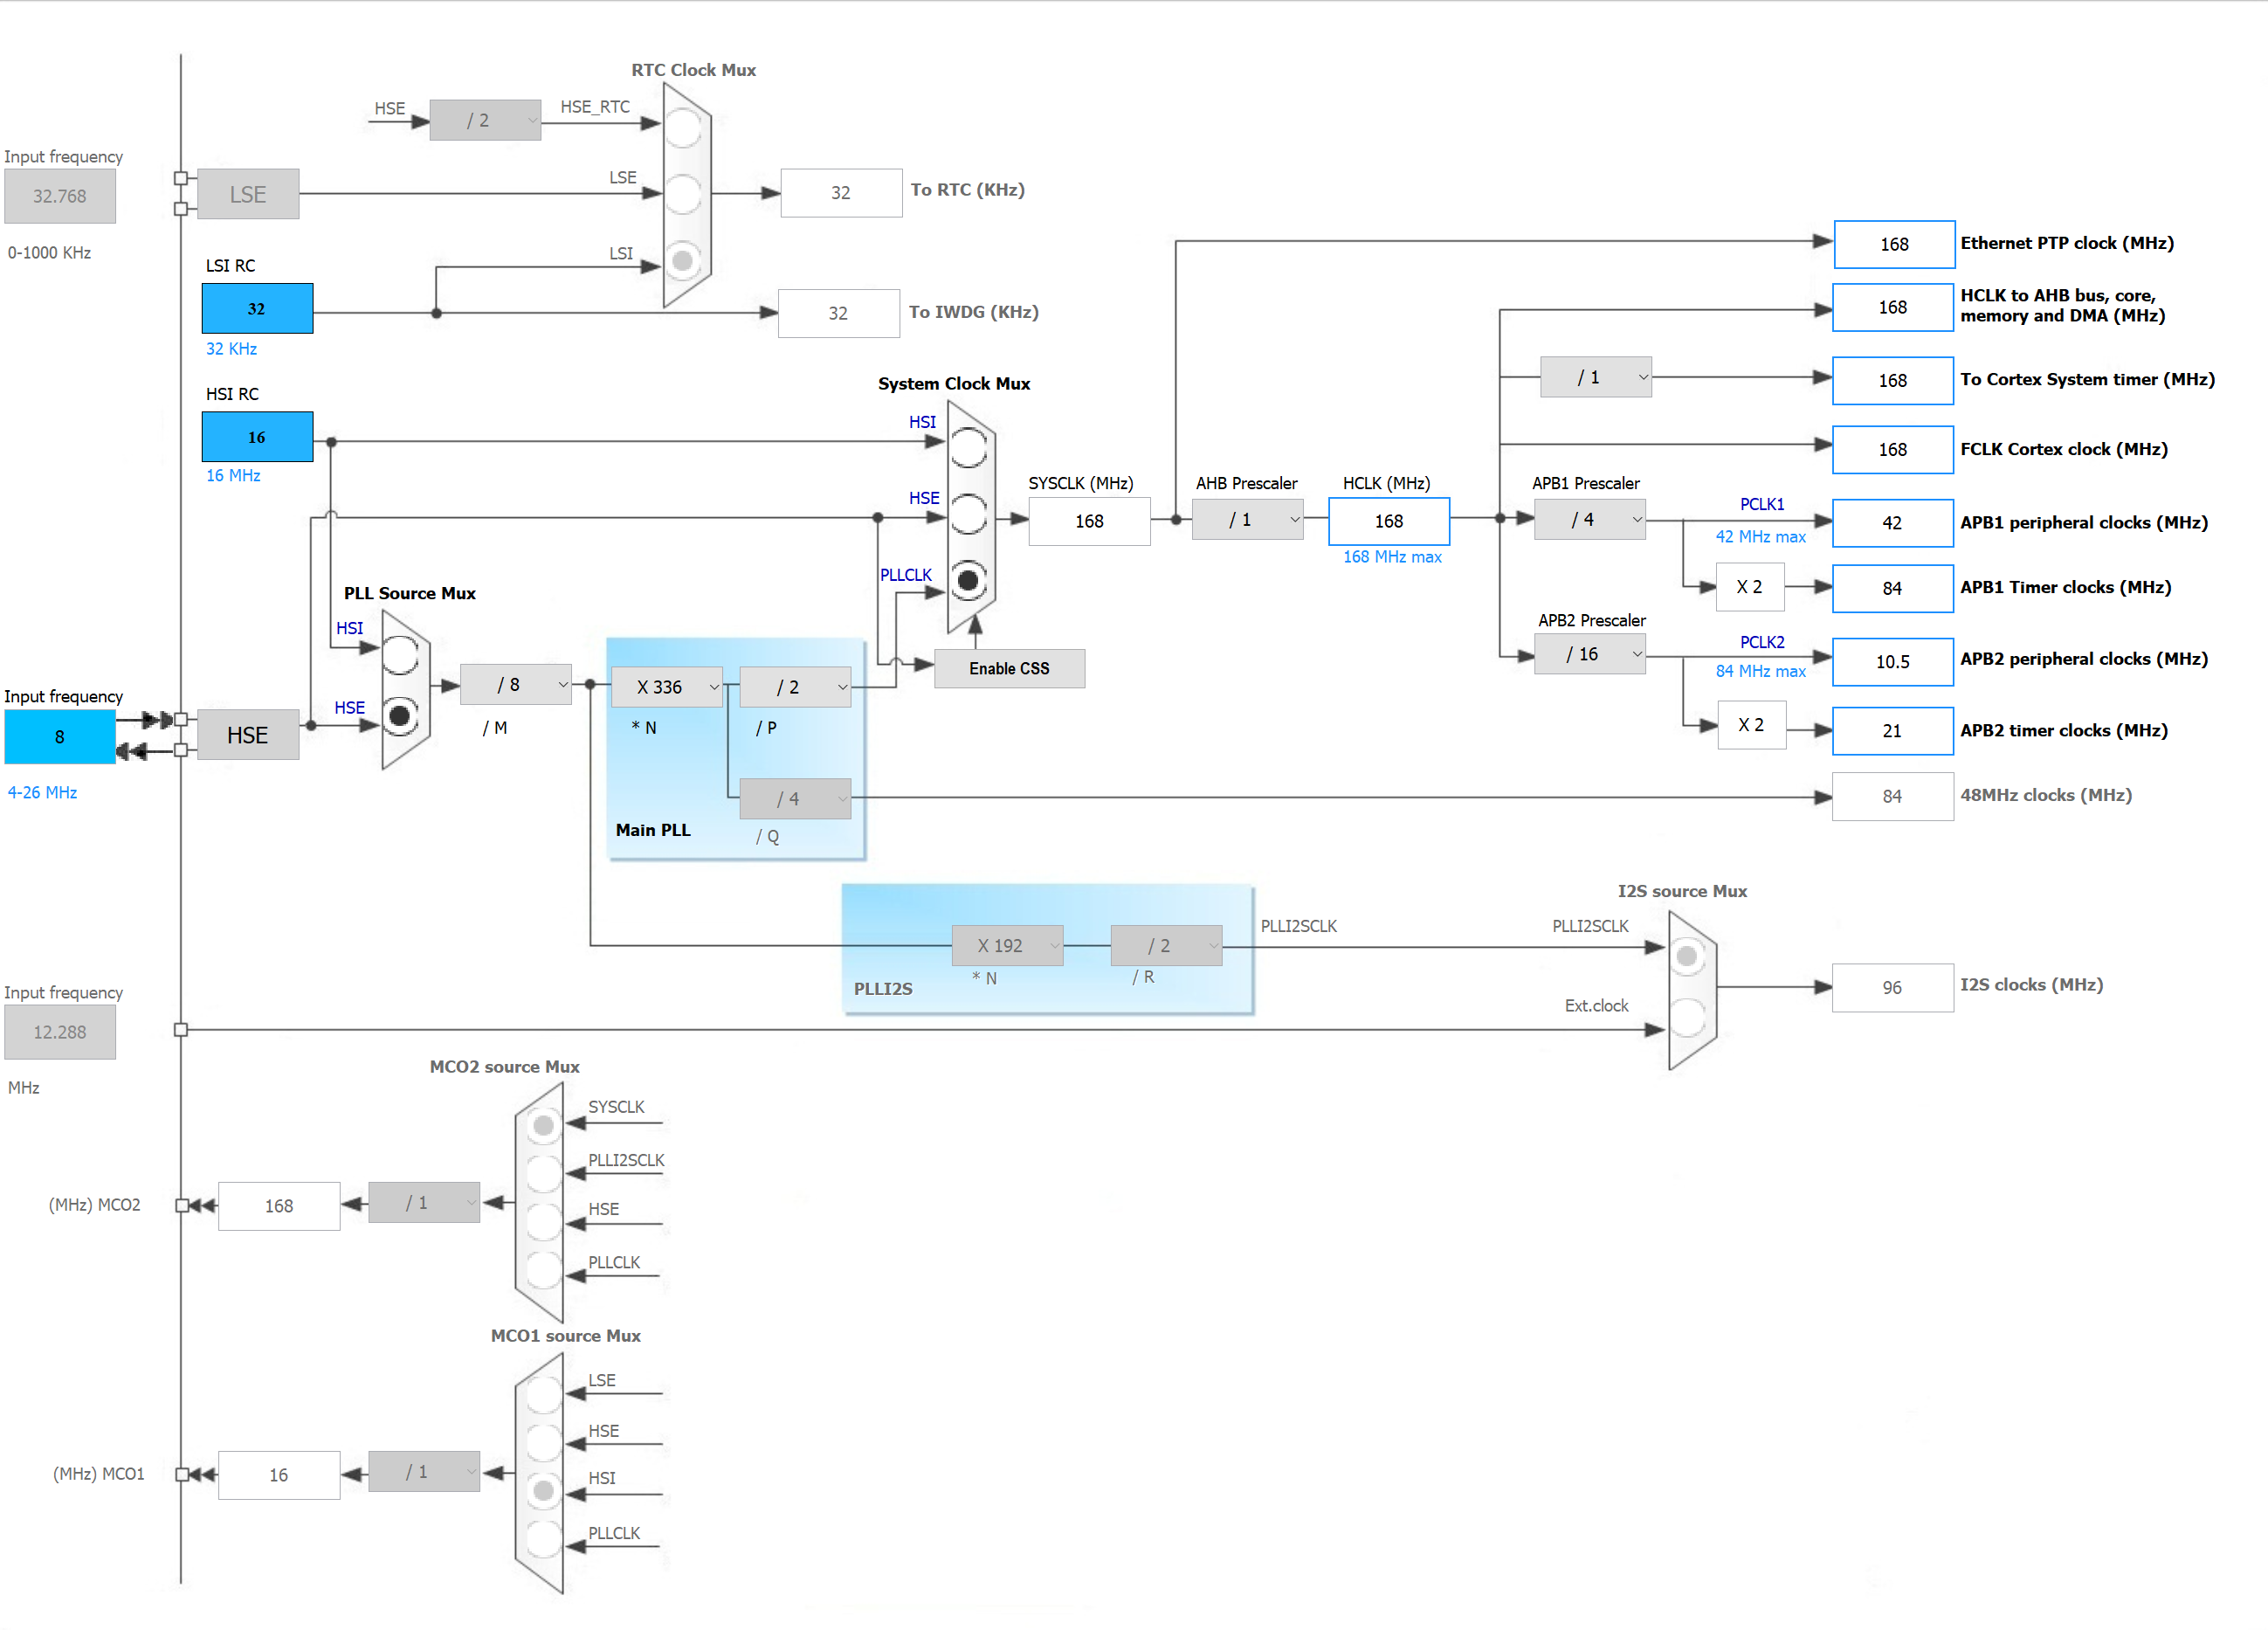
\includegraphics[width=\columnwidth]{./Bilder/fig_clock}%
\caption{Taktbaum generiert in STM32 CubeMX}%
\label{fig_clock}%
\end{figure}

\section{Einleitung in benutzerseitige CAN Schnittstelle} \label{CANNachrichten}

Für den späteren Anwender ist vornehmlich die Benutzerschnittstelle über CAN relevant. Hier wird zunächst zwischen drei Nachrichten unterschieden, die innerhalb des CAN-Netzwerkes fortlaufend ausgetauscht werden. Über die Nachricht \textit{TSA\_req}, die in \autoref{tab_tsa_req} beschrieben ist, kann ein übergeordnetes Steuergerät Befehle an den Aktor schicken. Diese werden dann abhängig des aktuellen Zustands entsprechend umgesetzt. Parallel werden vom Aktor permanent Nachrichten an das Steuergerät gesendet, die Informationen über den aktuellen Zustands liefern. Dabei werden die Informationen auf zwei Nachrichten aufgeteilt, genaueres ist \autoref{tab_tsa_trqs} und \autoref{tab_tsa_error} zu entnehmen. Das Gesamtkonzept ist in \autoref{fig_can_ov} dargestellt.

\begin{figure}[h]%
\centering
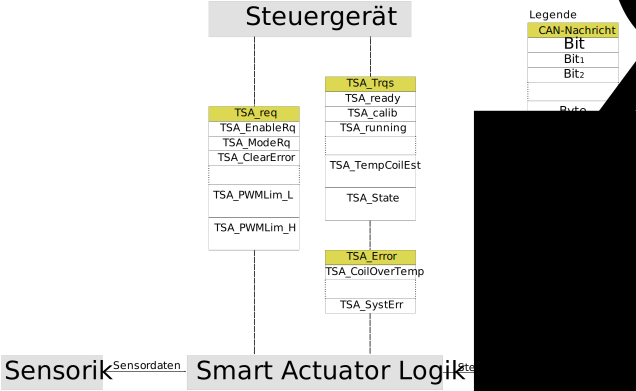
\includegraphics[width=0.6\columnwidth]{./Bilder/fig_can_ov}%
\caption{Gesamtkonzept der CAN-Kommunikation}%
\label{fig_can_ov}%
\end{figure}

\begin{table}%
\centering
\begin{tabular}{l c p{6cm} p{4cm}}
\hline
Bezeichnung & Datentyp & Erläuterung & Zusatz \\
\hline
TSA\_EnableRq & Bit & Aktivierungssignal des Aktors & Durch Setzen dieses Bits wird von Betriebsmodus \textbf{Inaktiv} zu \textbf{Regulär} gewechselt \newline \\
TSA\_ModeRq & Bit & Wahl des gewünschten Betriebsmodus \textbf{Regulär} oder  \textbf{Kalibrierung }& 0: Regulär, 1: Kalibrierung \newline \\
TSA\_ClearError & Bit & Fehler Quittierung & Durch Setzen wird von Betriebsmodus \textbf{Fehler} zu \textbf{Inaktiv} gewechselt, falls der Fehler behoben wurde \newline \\
TSA\_ShiftFirst & Bit & Schaltbefehl in ersten Gang & nur möglich in Betriebsmodus \textbf{Regulär} \newline\\
TSA\_ShiftSecond & Bit & Schaltbefehl in zweiten Gang & nur möglich in Betriebsmodus \textbf{Regulär} \newline \\
TSA\_ShiftNeutral & Bit & Schaltbefehl in neutrale Position & nur möglich in Betriebsmodus \textbf{Regulär} \newline \\
TSA\_PWMLim\_L & unsigned Byte & Obere Grenze für PWM - Puls/Pausen- Verhältniss & Low Byte \newline \newline \\
TSA\_PWMLim\_H & unsigned Byte & Obere Grenze für PWM - Puls/Pausen- Verhältniss & High Byte \\
\end{tabular}
\caption{Erläuterung der CAN-Nachricht \textit{TSA\_req}}
\label{tab_tsa_req}
\end{table}

\begin{table}%
\centering
\begin{tabular}{l c p{6cm} p{4cm}}
\hline
Bezeichnung & Datentyp & Erläuterung & Zusatz \\
\hline
TSA\_ready & Bit & Aktor ist betriebsbereit & Aktor befindet sich weder im Fehler- noch im Initialisierungszustand \newline \\
TSA\_calib & Bit & Laufender Kalibriervorgang & - \newline \\
TSA\_running & Bit & Warten auf Befehle & Aktor befindet sich in Betriebsmodus \textbf{Regulär} \newline \\
TSA\_shifting & Bit & Laufender Schaltvorgang & Es können keine weiteren Schaltbefehle entgegen genommen werden \newline\\
TSA\_firstGearEng & Bit & Erster Gang eingelegt & Gangposition erkannt und in gültigem Toleranzbereich \newline \\
TSA\_secondGearEng & Bit & Zweiter Gang eingelegt & Gangposition erkannt und in gültigem Toleranzbereich \newline \\
TSA\_neutralGearEng & Bit & Neutrale Gangposition eingelegt & Gangposition erkannt und in gültigem Toleranzbereich \newline \\
TSA\_Heartbeat& Bit & Lebenszeichen im Sekundentakt & Gibt Auskunft über funktionierenden Programmablauf \newline \newline \\
TSA\_Error & Bit & Fehlerzustand & Aktor in Betriebsmodus \textbf{Fehler}, Informationen liefert \textit{TSA\_Error} \newline \\
TSA\_ForkPosMeas & unsigned Byte & Aktuelle Schaltgabelposition & Gemessen in Millimetern \newline \\
TSA\_DcInput & unsigned Byte & Aktuelle Eingangsspannung & Gemessen in V \newline \\
TSA\_TempCoilEst & unsigned Byte & Aktuell gemessene Spulentemperatur & Gemessen in Grad Celsius, um +100 Offsetverschoben \newline \\
TSA\_State & unsigned Byte & Momentaner Zustand in Hauptzustandsautomaten & ID des Zustands des Hauptzustandsautomaten (zur Fehleranalyse) \\
\end{tabular}
\caption{Erläuterung der CAN-Nachricht \textit{TSA\_Trqs}}
\label{tab_tsa_trqs}
\end{table}

\begin{table}%
\centering
\begin{tabular}{l c p{6cm} p{4cm}}
\hline
Bezeichnung & Datentyp & Erläuterung & Zusatz \\
\hline
TSA\_CoilOverTemp & Bit & Übertemperatur in Spulenwicklungen festgestellt & Schwellwert konfigurierbar über \textit{ERR\_limCoilTemp} \newline \\
TSA\_HbridgeOvertemp & Bit & Übertemperatur in H-Brücke festgestellt & Schwellwert konfigurierbar über \textit{ERR\_limHTemp} \newline \\
TSA\_CalibErr & Bit & Fehlerhafte Kalibrierung & Timeout überschritten, ungültige Kalibrierergebnisse oder fehlerhafte Langzeitspeicherung \newline \\
TSA\_dcVErr & Bit &  Eingangsspannungsbereich unter- oder überschritten & Schwellwert konfigurierbar über \textit{ERR\_dcLimMin} und \textit{ERR\_dcLimMax} \newline \\
TSA\_SensErr & Bit & Fehlerhafte Sensormesswerte & Sensorwerte außerhalb des erwarteten Bereichs oder inkonsistent \newline \\
TSA\_ShiftErr & Bit & Fehler bei Schaltvorgang & Timeout überschritten oder unerwarter schlechter Schaltverlauf \newline \\
TSA\_ShortCirc & Bit &  Überstromerkennung in Aktor & Schwellwert konfigurierbar über \textit{ERR\_limCurrent} \newline \\
TSA\_SystErr& Bit & Ein Systemfehler ist aufgetreten & Softwaresystem befindet sich in ungeplantem Zustand und muss zurückgesetzt werden \newline \\

\end{tabular}
\caption{Erläuterung der CAN-Nachricht \textit{TSA\_Error}}
\label{tab_tsa_error}
\end{table}